\documentclass[wcp]{jmlr}

\usepackage{enumerate}
\usepackage{bbold}
\usepackage{booktabs}
\usepackage{natbib}
\usepackage[utf8]{inputenc}

 % The following command is just for this sample document:
\newcommand{\cs}[1]{\texttt{\char`\\#1}}


 % change the arguments, as appropriate, in the following:
%\jmlrvolume{1}
%\jmlryear{2014}
%\jmlrworkshop{\textcolor{red}{Neural Connectomics Workshop}}
\jmlrproceedings{}{}

\title{Simple connectome inference from partial correlation statistics in calcium imaging}

\author{Antonio Sutera,
        Arnaud Joly,
        Vincent François-Lavet,
        Aaron Qiu, \\
        Gilles Louppe,
        Damien Ernst,
        Pierre Geurts}

 % Authors with different addresses:
 % \author{\Name{Author Name1} \Email{abc@sample.com}\\
 % \addr Address 1
 % \AND
 % \Name{Author Name2} \Email{xyz@sample.com}\\
 % \addr Address 2
 %}

\editor{Editor's name}
 % \editors{List of editors' names}

\begin{document}

\maketitle

\begin{abstract}
In this work, we propose a simple and mathematically motivated method for the
problem of connectome inference in calcium imaging data. The proposed algorithm
consists in i) processing the raw signals to detect neural peak activities and ii)
inferring the degree of association between neurons from partial correlation
statistics.  This paper summarizes the methodology that led us to win the
Connectomics Challenge, proposes a simplified version of our method and finally
discusses our results with respect to other inference methods.
\end{abstract}

\begin{keywords}
Connectomics - Network inference - Partial correlation
\end{keywords}


\section{Introduction}\label{sec:intro}

The human brain is a complex biological organ made of 100 billions of neurons,
each connected to 7000 other neurons on average. Unfortunately, direct
observations of the connectome, the wiring diagram of the brain, is not yet
technically feasible. Without being perfect, calcium imaging currently allows
the realtime and simultaneous observation of neuron activities from thousands
of neurons, producing individual time series representing their fluoresence
intensity. In this context,  the connectome inference problem consists in
retrieving the synaptic connections between neurons on the basis of the
fluoresence time series. In particular, this problem is often made difficult
because of experimental issues, including masking effects making some of the
neurons not to be observed or confounded with others, a low sampling rate of
the optical device with respect to the neural activity speed or the slow decay
of fluoresence.

Formally, the connectome can be represented as a directed graph $G=(V,E)$,
where $V$ is a set of $p$ nodes, representing neurons, and $E \subseteq
\left\{(i, j) \in V \times V\right\}$ is a set of edges, representing direct
synaptic connections between neurons. Causal interactions are expressed by the
direction of edges: $(i, j) \in E$ indicates that the state of neuron $j$ might
be caused by the activity of neuron $i$. In those terms,  the connectome
inference problem is formally stated as follows:  \textit{Given the sampled
observations $\{ x^t_i \in \mathbb{R}^{p} | i \in V, t = 1, \dots T \}$ of $p$
neurons for $T$ time intervals, the goal is to infer the set $E$ of connections in $G$.}

In this paper, we present a simplified -- yet nearly as good -- version of
the winning method\footnote{Code available at \url{https://github.com/asutera
/kaggle-connectomics}} of the Connectomics
Challenge\footnote{\url{http://connectomics.chalearn.org}}, as a simple and
theoretically grounded approach based on signal processing techniques and
partial correlation statistics. The rest of the paper is structured as
follows: Section \ref{sec:filter} describes the signal processing methods
applied on fluorescent calcium time series; Section \ref{sec:inference} then
presents the proposed approach and its theoretical properties; Section
\ref{sec:results} provides an empirical analysis and comparison with other
network inference methods, while Section \ref{sec:conclusion} finally
discusses our work and provides further research directions. Additionnaly, Appendix
\ref{app:optimized} further describes our actual winning method, giving slightly
better results than the method presented in the paper but highly tuned for the
challenge.


\section{Signal processing} \label{sec:filter}

Under the simplifying assumption that neurons are on-off units, characterized
by short periods of intense activities, or peaks, and longer periods of
inactivity, the first part of our algorithm consists in cleaning the raw
fluoresence data. More specifically, time series are processed using standard
signal processing filters in order to remove noise due light scattering
effects, account for fluorescence  low decay and reduce the importance of
global high activity in the network. The overall process is illustrated on
Figure~\ref{fig:filtered-signal}.

\begin{figure}
\centering
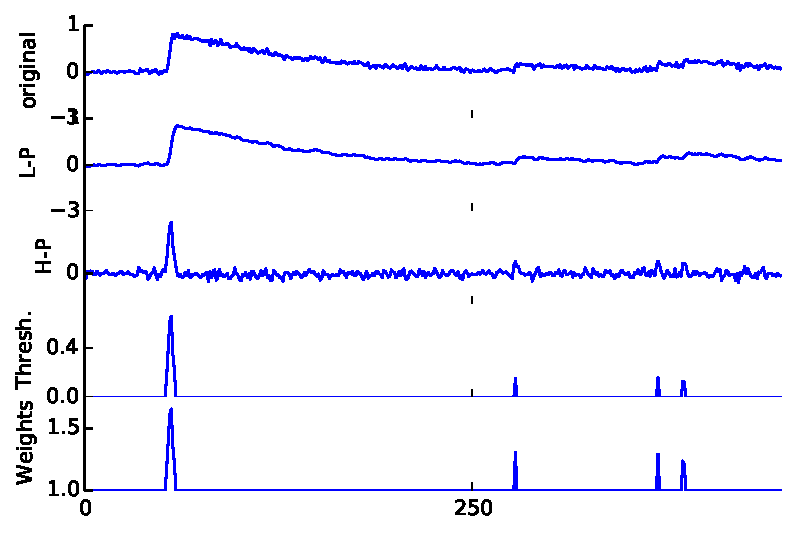
\includegraphics[width=0.4\linewidth]{images/fig_filtering}
\caption{Signal processing process.}
\label{fig:filtered-signal}
\end{figure}



As the first plot in Figure~\ref{fig:filtered-signal} illustrates, due to
light scattering artifacts that ordinarily affects the quality of the
recording~\citep{lichtman2011big}, the raw fluoresence signal is very noisy.
Accordingly, the first step of our pipeline is to smoothen the signal, using a low-pass filter for
filtering out high frequency noise, applying one of the following designs and
resulting in the second plot in the figure:
\begin{align}
% symmetrical median filter
x^t_i &\leftarrow x^{t-1}_i + x^{t}_i + x^{t+1}_i \label{eq:symetric-median}, \\
% asymmetrical weighted median
x^t_i &\leftarrow 0.4 x^{t-3}_i + 0.6 x^{t-2}_i + 0.8 x^{t-1}_i + x_{t}^i.
\label{eq:weighted-asymetric-median}
\end{align}

Considering the short delay of communication between neurons and the slow
decay of fluorescence, the second step of our pipeline consists in identifying
neuron spikes -- characterized by high frequencies -- by filtering out low
frequencies through a high-pass filter, resulting in third plot of the figure:
\begin{align} % an asymmetrical discrete derivative filter 
x^{t,d}_{i} &\leftarrow x^{t}_i - x_{t-1}^i. \label{eq:high-pass-filter} 
\end{align}

Once the low- and and high-pass filters have been applied, the remaining signal
corresponds to the discrete derivative of the fluorescence time series. To
further filter out small signal variations, mostly due to noise, the third step
consists in a  hard-threshold filter, yielding the fourth plot in the figure:
\begin{align}
x^{t,d}_i &\leftarrow x^{t,d}_i \mathbb{1}(x^{t,d}_i \geq \tau) \text{ with } \tau > 0.
\end{align}

At this step, the processed signal only contains clean spikes. However, when a
large part of the network is firing, detecting pairwise neuron interactions is a
difficult task. \textcolor{red}{G: say that neurons may fire because of global
high activity, without any actual cause -- see generator.}
Accordingly, in order to reduce false interaction detection,
peak intensities at time $t$ are regularized by the global activity of all
neurons, thereby reducing the importance of peaks identified during global high activity periods:
\begin{align}
 x^{t,w}_i  &\leftarrow (x^{t,d}_i + 1 )^{1 + \frac{1}{\sum_{j} x^{t,d}_j}}.
\end{align}


\textcolor{red}{G: Change notations for $f(x^t) = ...$, $g(x^t) = ...$}

\section{Connectome inference from partial correlation statistics}
\label{sec:inference}

Let us denote the fluorescence calcium indicators of all neuron
as a set of random variables $X = \left\{X_1, \ldots, X_{|V|}\right\}$, which follows
a joint probability distribution $p_\mathcal{X}$, and by
$X^{-i,j}$ the set of all variables except $X_i$ and $X_j$.
Two random variables $X_i$ and $X_j$ are said to be conditionally independent
to a (possibly empty) set of random variables $Z$, denoted by $X_i \perp X_j | Z$,
if the joint conditional probability distribution factorizes
$p_{\mathcal{X}_i, \mathcal{X}_j|\mathcal{Z}} = p_{\mathcal{X}_i|\mathcal{Z}}
p_{\mathcal{X}_j|\mathcal{Z}}$.  The inference of the undirected network
can be formulated as inferring conditional dependences
$X_i \not\perp X_j | X^{-i,j}$ between all pairs $i$ and $j$ of fluorescence
signals.


Since all neurons are assumed to form a connected graph, we
have by construction $X_i \not\perp X_j$. However, two random variables $A$ and $B$ might be
dependent taken alone ($A \not\perp B$), but not once we observe the set  $C$
of all other variables ($A \perp B | C$). The conditioning over all other
random variables $X^{-i,j}$ is thus necessary to avoid predicting an edge when
two neurons are not directly connected.

If the random variables $X$ follows a joint Gaussian distribution
$p_\mathcal{X} \sim \mathcal{N}(\mu; \Sigma)$ of mean vector $\mu$ and
covariance matrix $\Sigma$, we have the conditional independence
$X_i \perp X_j | X^{-i,j}$ if the partial correlation coefficient
\[
\rho_{X_i, X_j | X^{-i,j}}
= \frac{\Sigma^{-1}_{ij}}{\sqrt{\Sigma^{-1}_{ii} \Sigma^{-1}_{jj}}}
\]
is equal to zero \citep{koller2009probabilistic}. The partial correlation gives
an estimate of the degree of association between all
pairs of neuron $i$ and $j$. 
Similarly, we also have $X_i \perp X_j$ if the Pearson correlation
coefficient
\[
\rho_{X_i,X_j} = \frac{\Sigma_{ij}}{\sqrt{\Sigma_{ii}
\Sigma_{jj}}}
\]
is equal to zero.

% Speak about why averaging
The quality of the signal filtering and network inference depends on
good hyper-parameter selection, which are themselves dependent on the properties
of the targeted network and measurement conditions, e.g. signal to noise ratio.
In order to improve robustness, a weighted average of partial correlation
matrices was estimated from the time series by varying the hard-threshold value
$\tau$ and the design of the low-pass filter (mentionned in section \ref{sec:filter} and appendix \ref{app:optimized}).


\textcolor{red}{Say that we use PCA to derive the precision matrix + ref!.}

Finally since there is a high correlation between neurons,
we filter some more noise through a principal component analysis. From the $|V|$
eigen vectors, we kept $80\%$ of the eigen vectors which have the largest eigen
value. In the context of the challenge, this assumption was deduced from ground
truth of provided networks.


\section{Experiments}
\label{sec:results}

% Datasets
To assess our method, we have used four datasets provided by the organizers
of the Connectomics challenge : \textit{normal-1, normal-2, normal-3, normal-4}.
Those datasets are time series of size $T=179500$ of image calcium from simulated
neuronal networks \citep{stetter2012model} with $|V|=1000$ neurons. The networks
to inferred have around 15000 edges and are similar to those
used to rank challenge participants.

% Metrics : ROC AUC and AUPRC
In supervised learning terms, the network inference task can be viewed as a
binary classification task where one has to correctly classify the presence
or the absence of edges of the graph. We assess the accuracy of the
network inference method using the area under the ROC curve (AUROC)
and the area under the precision-recall curve (AUPRC)
\citep{schrynemackers2013protocols}. Since neurons are not self-connected
($(i, i) \not \in E, \forall i \in V$) and some inference methods could
give maximal scores to the diagonal of $\hat{A}$, e.g. Pearson
correlation, we set those elements to the minimum of $\hat{A}$ prior
assessment.


% TODO
%   - discussions about the results
%   - discussions about the metrics (Gilles' text)

% For the directory method, only filters defined by Equations
% \ref{eq:low-pass}, \ref{eq:high-pass} and \ref{eq:hard-treshold-filter} were
% used.


% Dummy classifier?


% GTE : Explaning the method (default parameters!)

% Explaining the method (thèse de Gilles)
% Genie3 : better in auprc while worse in auroc than GTE. Why?
% Genie3 : "Conditioning" better and better but need a lot of trees
% Correlation : Already give good results

% Partial correlation : Obvious improvements (both metric) because of the conditioning

% Directivity : ?


%Opt: obviously when parameters are tuned/optimized, it's slightly better --> see appendix for a full description of the method
% Avg.: Averaging over the threholds and L-P filters improves a lot both metrics.

GTE is a method which characterizes a relationship between neurons by an
estimation of the generalized transfer entropy \citep{stetter2012model}. The
goal of this method tries to see if the next time step value is better from
the previous values of this time series or from time series of other neurons.

GENIE3 is a tree-based method which sees the network inference problem as $p$,
the number of variables, independent supervised learning problems (todo cite:
Irrthum?Van Anh?Pierre?). Formally, each sub-problem consists in the
prediction of one variable, the target, from the remaining $p-1$ variables.
This method uses random forests to estimate the target variable and variable
importances can be derived to estimate the adjacency matrix $A$ (see (todo
cite) for a more detailed description of the inference method).

At first sight, it appears on Tab.\ref{tab:tab1} that partial
correlation outperforms other methods. Two main reasons may explain this.
First, the quality of the infered network seems related to the conditioning
part of the method. In every method except with partial correlation, indirect
links are confounded with direct links.  Secondly, the gaussian assumption
seems verified and thus linear method appears to be competitive, e.g. the
method correlation already gives good results, with a non-linear method such
as GENIE3.\\

% Discussion about the metrics Observing Tab.\ref{tab:tab1}, it appears that
best methods only infer the \textbf{undirected} network by giving the same
weights to both edges $(i,j)$ and $(j,i)$. This is quite surprising
considering the goal of the challenge, namely predicted directed connections
between neurons. Besides, if the true network undirected, i.e. for all links
$(i,j)$, back links are added, is the infered network then the score obtained
according to the ROC AUC metric is very high ($\sim 0.9956$ on
\textit{normal-1}). Therefore, an undirected infered network seems sufficient
to maximize the ROC AUC score without trying to identify the link direction.
Indeed, predicting perfectly directivity only yields a small gain ($\sim
0.005$ on \textit{normal-1}) which is is not very rewarding. In contrast, the
same experiment with the precision recall metric rewards less the undirected
network and the gain margin in predicting the link directivity is large enough
to be interesting. For these reason, it seems that the metric used in the
contest, i.e. the ROC AUC, does not seem consistent with the goal of
predicting directed connections between neurons. Another metric, such as the
AUC PRC, is maybe more appropriate to assess the quality of the
\textbf{directed} infered network.

Interestingly, an easy way to improve results for asymmetric method (see Tab.\ref{tab:tab2}), namely GTE and GENIE3, is to make undirected the infered network. 

\begin{table}
\small
\centering
\begin{tabular}{@{}l *{8}{c}@{}}
  & \multicolumn{4}{c}{AUROC} & \multicolumn{4}{c}{AUPRC} \\
\cmidrule(r){2-5}\cmidrule(r){6-9}
Methods $\backslash$ normal- & 1 & 2 & 3 & 4 & 1 & 2 & 3 & 4 \\
\hline \hline
% Directivity \textcolor{red}{appendix?} & 0.535 & 0.526 & 0.533 & 0.535 & 0.012 & 0.012 & 0.012 & 0.012 \\
Correlation            & 0.886 & 0.884 & 0.891 & 0.877 & 0.153 & 0.145 & 0.170 & 0.132 \\
GENIE3 (depth = 1)     & 0.878 & & & & 0.184 & & & \\
GENIE3 (depth = 2)     & 0.889 & & & & 0.217 & & & \\
GENIE3 (depth = 3)     & & & & & & & & \\
GTE                    & 0.890 & 0.893 & 0.894 & 0.873 & 0.171 & 0.174 & 0.197 & 0.142 \\
Partial correlation    & 0.930 &  0.927 &  0.926 &  0.923& 0.363  & 0.347 &  0.346 & 0.328 \\
Partial correlation (opt.) & 0.932 & 0.931 & 0.930 & 0.928 & 0.364 & 0.366 & 0.359 & 0.344 \\
Our approach (opt. \& avg.)    & 0.943 & 0.942 & 0.942 & 0.939 & 0.403 & 0.404 & 0.398 & 0.388 \\
% Our approach + dir  \textcolor{red}{appendix?}   & 0.944 & 0.943 & 0.942 & 0.940 & 0.404 & 0.405 & 0.399 & 0.389 \\
\end{tabular}
\caption{TODO}
\label{tab:tab1}
\end{table}


\begin{table}
\small
\centering
\begin{tabular}{@{}l *{8}{c}@{}}
  & \multicolumn{4}{c}{AUROC} & \multicolumn{4}{c}{AUPRC} \\
\cmidrule(r){2-5}\cmidrule(r){6-9}
Methods $\backslash$ normal- & 1 & 2 & 3 & 4 & 1 & 2 & 3 & 4 \\
\hline \hline
% Directivity \textcolor{red}{appendix?} & 0.535 & 0.526 & 0.533 & 0.535 & 0.012 & 0.012 & 0.012 & 0.012 \\
GENIE3 (depth = 1)     &  & & & & & & & \\
GENIE3 (depth = 2)     &  & & & & & & & \\
GENIE3 (depth = 3)     &  & & & & & & & \\
GTE                    &  & & & & & & & \\
% Our approach + dir  \textcolor{red}{appendix?}   & 0.944 & 0.943 & 0.942 & 0.940 & 0.404 & 0.405 & 0.399 & 0.389 \\
\end{tabular}
\caption{TODO (network are undirected)}
\label{tab:tab2}
\end{table}



\begin{table}[tbh]
\centering
\caption{TODO}
\begin{tabular}{@{}l *{8}{c}@{}}
  & \multicolumn{4}{c}{AUROC} & \multicolumn{4}{c}{AUPRC} \\
\cmidrule(r){2-5}\cmidrule(r){6-9}
Methods $\backslash$ normal- & 1 & 2 & 3 & 4 & 1 & 2 & 3 & 4 \\
\midrule
No  filtering       & 0.777 & 0.767 & 0.772 & 0.774 & 0.070 & 0.064 & 0.068 & 0.072\\
P                   & 0.925 & 0.925 & 0.924 & 0.923 & 0.322 & 0.324 & 0.323 & 0.312\\
P + W               & 0.931 & 0.930 & 0.928 & 0.927 & 0.333 & 0.334 & 0.327 & 0.313\\
P + W + PCA         & 0.932 & 0.931 & 0.930 & 0.928 & 0.364 & 0.366 & 0.359 & 0.344\\
Averaging           & 0.943 & 0.942 & 0.942 & 0.939 & 0.403 & 0.404 & 0.398 & 0.388\\
Averaging + Directivity & 0.944 & 0.943 & 0.942 & 0.940 & 0.404 & 0.405 & 0.399 & 0.389\\
\end{tabular}
\end{table}





\section{Conclusions} \label{sec:conclusion}

In previous study \citep{shipley2002cause}, it has been suggested to
consider correlation coefficients of all possible orders,
i.e. conditioned on every subsets of the set of $p-2$ other variables. This
would take into account multiple indirect paths between a given pair of
variables.

% Possible extensions
% partial autocorrelation function (sometimes "partial correlation function")
% conditional independence test
% Speak about the complexity and parallelization of the methods





\section*{Acknowledgements}

A. Joly and G. Louppe are research fellows of
the FNRS, Belgium.  A. Sutera is  is recipient of
a F.R.I.A. fellowship of F.R.S.-FNRS, Belgium.
This work is supported by PASCAL2 and the IUAP DYSCO, initiated by the
Belgian State, Science Policy Office.



\newpage
\clearpage

% We allow the bibliography to be added on top of the 6 pages.
% Supplementary material may be added in the form or a URL pointed to from
% the paper.
\bibliography{references}

\newpage
\clearpage

\appendix


\section{An optimized version of the algorithm to win the challenge}
\label{app:optimized}


The algorithm propose in sections \ref{sec:filter} and \ref{sec:inference} has been optimized at its extreme limit to win the challenge. In this section, we will describe the full tuned algorithm and present some results.

Note that our parameter tuning was mainly
done on the \textit{normal-1} dataset and partly on \textit{normal-4} dataset,
therefore it may justify why these networks are better retrieved despite the
fact that some might be simpler to infer.

% Introduce a custom solution to make the Y matrix asymmetric
% Introduce directivity
\textcolor{red}{Est-ce qu'on ne le ferait pas passer dans l'appendice B? Ou du moins l'équation?}
Since partial correlation is a symmetric measure, the causal mechanism behind the
interaction ($A$ directly causes $B$, $B$ directly causes $A$ or both) can not
be directly inferred\footnote{Also note that two other causal mechanisms might be
implied while having a non-zero partial coefficient: (i) a pair of variables
is induced by a common (hidden) variable; (ii) $A$ (respectively $B$) is
conditionally correlated to a hidden variable affecting $B$ (resp. $A$)
\citep{de2004discovery}.}.
In order to retrieve causal information, we developed an
heuristics based on the following observation. The rise of fluorescence
indicates the activation of a neuron $i$. If a neuron $j$ have also
an increased of fluorescence after a slight delay, this could have been
caused by the neuron $i$. Thus, we count whenever
such events occurred between consecutive time steps
\[
\hat{Z}: z_{ij} = \sum_{t=1}^{T - 1}
    \mathbb{1}(x_j^{t+1} - x_i^t \in \left[f_1, f_2 \right]) -
    \mathbb{1}(x_i^{t+1} - x_j^t \in \left[f_1, f_2 \right]), \forall i, j \in V
\]
where $f_1$ and $f_2$ are parameters of the method.
Finally, the weighted average of correlation matrices is combined with $Z$ such
that $Z$ has a contribution of $0.3\%$ to the prediction of an edge.

\section{Supplementary results}

\begin{table}[htbp]
\centering
\caption{Correlation (ROC). Improvement of each stage of our approach. Note that we choose the
         \textit{best} threshold (\textcolor{red}{for now 0.11}) for stages 1 to 4.}
\begin{tabular}{*{5}{l}}
\toprule
Stage               & normal-1 & normal-2 & normal-3 & normal-4 \\
\midrule
Nothing             & 0.681 & 0.699 & 0.683 & 0.681\\
Weights             & 0.695 & 0.713 & 0.697 & 0.694\\
H-T                 & 0.876 & 0.873 & 0.877 & 0.869\\
H-T + Weights       & 0.886 & 0.884 & 0.891 & 0.877\\
P-P                 & 0.857 & 0.850 & 0.843 & 0.832\\
P-P + Weights       & 0.826 & 0.823 & 0.817 & 0.799\\
\bottomrule
\end{tabular}
\end{table}

\begin{table}[htbp]
\centering
\caption{Correlation (P-R). Improvement of each stage of our approach. Note that we choose the
         \textit{best} threshold (\textcolor{red}{for now 0.11}) for stages 1 to 4.}
\begin{tabular}{*{5}{l}}
\toprule
Stage               & normal-1 & normal-2 & normal-3 & normal-4 \\
\midrule
Nothing             & 0.028 & 0.028 & 0.025 & 0.026\\
Weights             & 0.031 & 0.030 & 0.027 & 0.028\\
H-T                 & 0.143 & 0.128 & 0.150 & 0.129\\
H-T + Weights       & 0.153 & 0.145 & 0.170 & 0.132\\
P-P                 & 0.100 & 0.087 & 0.079 & 0.083\\
P-P + Weights       & 0.079 & 0.071 & 0.067 & 0.064\\
\bottomrule
\end{tabular}
\end{table}

\begin{table}[htb]
\centering
\caption{Comparison (P-R) with other methods (for now, $t = 0.11$)}
\begin{tabular}{*{5}{l}}
\toprule
Methods             & normal-1 & normal-2 & normal-3 & normal-4 \\
\midrule
Correlation (best)         & 0.153 & 0.145 & 0.170 & 0.132 \\
Partial correlation (best) & 0.364 & 0.366 & 0.359 & 0.344 \\
Our approach (best)        & 0.403 & 0.404 & 0.398 & 0.388 \\
GENIE3                     & & & & \\
GTE                        & 0.171 & 0.174 & 0.197 & 0.142 \\
Directivity                & 0.012 & 0.012 & 0.012 & 0.012 \\
Our approach + dir         & 0.404 & 0.405 & 0.399 & 0.389 \\
\bottomrule
\end{tabular}
\end{table}

\begin{table}[htb]
\centering
\caption{Inverse correlation (ROC). Improvement of each stage of our approach. Note that we choose the
         \textit{best} threshold (\textcolor{red}{for now 0.11}) for stages 1 to 4.}
\begin{tabular}{*{5}{l}}
\toprule
Stage               & normal-1 & normal-2 & normal-3 & normal-4 \\
\midrule
Nothing             & 0.777 & 0.767 & 0.772 & 0.774 \\
PCA                 & 0.780 & 0.770 & 0.776 & 0.777 \\
Weights             & 0.780 & 0.769 & 0.776 & 0.777 \\
Weights + PCA       & 0.783 & 0.772 & 0.779 & 0.780 \\
H-T                 & 0.893 & 0.891 & 0.891 & 0.886 \\
H-T + PCA           & 0.894 & 0.892 & 0.891 & 0.886 \\
H-T + Weights       & 0.899 & 0.897 & 0.896 & 0.891 \\
H-T + Weights + PCA & 0.900 & 0.898 & 0.896 & 0.892 \\
P-P                 & 0.925 & 0.925 & 0.924 & 0.923 \\
P-P + PCA           & 0.926 & 0.926 & 0.925 & 0.923 \\
P-P + Weights       & 0.931 & 0.930 & 0.928 & 0.927 \\
P-P + Weights + PCA & 0.932 & 0.931 & 0.930 & 0.928 \\
Averaging (PCA)     & 0.943 & 0.942 & 0.942 & 0.939 \\
Stacking            & 0.944 & 0.943 & 0.942 & 0.940 \\
\bottomrule
\end{tabular}
\end{table}

\begin{table}[htb]
\centering
\caption{Inverse correlation (P-R). Improvement of each stage of our approach. Note that we choose the
         \textit{best} threshold (\textcolor{red}{for now 0.11}) for stages 1 to 4.}
\begin{tabular}{*{5}{l}}
\toprule
Stage               & normal-1 & normal-2 & normal-3 & normal-4 \\
\midrule
Nothing             & 0.070 & 0.064 & 0.068 & 0.072\\
PCA                 & 0.076 & 0.070 & 0.075 & 0.079\\
Weights             & 0.074 & 0.067 & 0.072 & 0.076\\
Weights + PCA       & 0.080 & 0.073 & 0.079 & 0.083\\
H-T                 & 0.264 & 0.260 & 0.269 & 0.241\\
H-T + PCA           & 0.266 & 0.263 & 0.273 & 0.244\\
H-T + Weights       & 0.280 & 0.273 & 0.281 & 0.251\\
H-T + Weights + PCA & 0.284 & 0.278 & 0.285 & 0.255\\
P-P                 & 0.322 & 0.324 & 0.323 & 0.312\\
P-P + PCA           & 0.347 & 0.352 & 0.355 & 0.341\\
P-P + Weights       & 0.333 & 0.334 & 0.327 & 0.313\\
P-P + Weights + PCA & 0.364 & 0.366 & 0.359 & 0.344\\
Averaging           & 0.403 & 0.404 & 0.398 & 0.388\\
Stacking            & 0.404 & 0.405 & 0.399 & 0.389\\
\bottomrule
\end{tabular}
\end{table}



%% Talk about filters future and past

\end{document}

